
\section{Web layout}

Web pages are written in HTML,
  which is a tree-structured markup language
  containing text and elements that wrap it.
The web browser's parsed representation of this tree
  is called the DOM or HTML tree.
To draw the page to the screen,
  the browser applies a sequence of transformations---%
  called rendering phases---%
  to this DOM tree: matching, styling, layout, paint, and so on.
The focus of this paper, the layout phase,
  applies to an intermediate tree structure
  called a ``layout tree'',
  whose shape largely matches the DOM tree
  (though with some deviations for ``generated content''
  like bullets for list items).
The layout phase reads layout node properties
  (which reflect HTML attributes, CSS properties, and other data)
  and computes layout fields like width and height for those nodes.
Later phases like painting then read those layout fields
  and use them to draw the page to the screen.
The DOM and layout trees are typically poorly-balanced,
  with both lots of ``wrapper'' elements (with a single child)
  and also many ``list'' elements with many children;
  an example DOM tree for a small web page
  is shown in Figure~\ref{fig:dom-tree-db}.
In memory,
  the layout tree is stored as a pointer tree,
  with the children stored as a doubly linked list,
  to allow for fast insertions and deletions.
This pointer-heavy structure means
  that layout nodes are spread throughout memory,
  with every access typically generating a cache miss.

\subsection{The Layout Phase}

The layout phase computes a number of layout fields
  for each node in the layout tree.
Computing layout fields is a recursive process
  because each node's layout depends on the layout of its neighbors.
For example, the height of a node is (typically)
  the sum of the heights of all its children,
  while a node's $x$ position depends on the $x$ position
  of its previous sibling, plus that previous sibling's width.%
\footnote{
  In reality, these rules are quite a bit more complex,
    with various exceptions to the simplified sketch given here.
}
Moreover, visible properties like width and height
  in turn depend on intermediate properties such as intrinsic size,
  current line ascent/descent, and even more obscure properties
  like the sum of its siblings' \texttt{flex-grow} values.
A complete layout phase must visit each node multiple times,
  in a well-defined order,
  in order to compute each field on each node
  before any others that depend on it.

\begin{figure}
\begin{minipage}[b]{0.68\linewidth}
\begin{verbatim}
# real web layout much more complex
def layout_simple(self): 
  self.width <-
    if parent? then max(0, parent.width - 10)
    else 50 # screen size
  children.forEach(layout_simple)
  self.height <-
    if last? then last.height_acc + 10 # padding
    else self.attribute[height]
  self.height_acc <-
    if prev?
    then prev.height_acc + self.height + 10 # margin
    else 0
\end{verbatim}
\caption{A layout algorithm that computes width and height of each dom node. The above program is a tree traversal: it walks down the tree then walks up the tree, computing values for each node during the walk.}
\label{fig:layout-simple}
\end{minipage}\hfill%
\begin{minipage}[b]{0.28\linewidth}
\centering
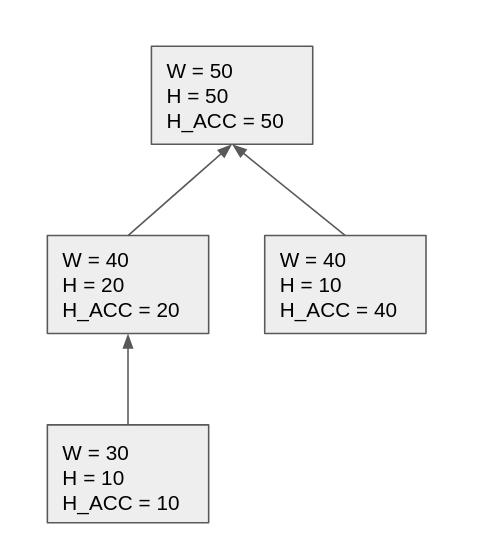
\includegraphics[scale=0.23]{LayoutExample.png}
\caption{The layout algorithm running on a layout tree of size 4. All nodes have an height attribute of 10.}
\end{minipage}
\end{figure}

We remark on a couple of key properties of layout
  that influence our approach:
\begin{enumerate}
\item Bounded work per node. There are no
  data-dependent loops, recursions, or data structures
  except the layout tree itself.
\item Immutable shape. The layout tree's structure
  is not modified during layout;
  only the layout fields on each node are.
Moreover, these computed fields
  are only written once (per frame)
  and then become read-only (for that frame).
\item Static control flow.
  The fields are computed in a fixed order
    dependent only on the layout tree shape,
    not the values of other computed fields.
\item Local data flow.
  To compute a particular node's fields,
    only that node's neighbors in the layout tree
    and their fields are accessed.
\end{enumerate}
These properties are discussed in
  the wealth of prior work on formalizing layout%
  ~\cite{meyerovich-1,meyerovich-2,meyerovich-3,cassius-1,cassius-2,cassius-3,yufeng-1,yufeng-2}.

In other words, layout can be expressed in the DSL
  shown in Figure~\ref{fig:dsl}.
In this DSL, a layout is defined by a set of passes
  $\text{Pass}_n$ performed in a certain order (the schedule).
Each pass performs a recursive, in-order traversal of the tree,
  computing some fields pre-order and some fields post-order.
Each field computation is a simple assignment $\mathsf{self}.V \gets T$,
  where $V$ is a field of the current node $\mathsf{self}$
  and $T$ is an expression that can refer to
  fields of $\mathsf{self}$ or its neighbors
  $\mathsf{parent}$, $\mathsf{prev}$, $\mathsf{next}$,
  $\mathsf{first}$ child, and $\mathsf{last}$ child.
Computations can also refer to HTML attributes or CSS properties
  of the current node
  using $\mathsf{attribute}[x]$ or $\mathsf{property}[x]$.%
\footnote{
We use two different namespaces
  for HTML attributes and CSS properties
  because some names, like \texttt{height},
  appear in both sets.
There is no other semantic difference between them,
  and other accessible properties,
  such as the tag name or image width and height
  do not affect invalidation traversal
  (but are modeled in our system as special properties).
}
Expressions can also use conditionals
  to test whether a given neighbor exists ($\mathsf{N?}$).
Notably, our DSL enforces
  the key properties of layout described above:
  there is no functionality to mutate the tree shape
  or to reorder control flow according to field values.
There are also no loops or data structures,
  and the only field access allowed is to a node's neighbors.

Many compound operations can be compiled into this DSL;
  for example, to access $\mathsf{parent}.\mathsf{parent}.\mathsf{x}$,
  one can instead define
  $\mathsf{self}.\mathsf{parent\_x} \gets \mathsf{parent}.x$
  to store each node's parent's $x$ field.
Then $\mathsf{parent}.\mathsf{parent}.x$
  is simply $\mathsf{parent}.\mathsf{parent\_x}$.
In any case, prior work in similar DSLs%
  ~\cite{meyerovich-1, meyerovich-2, cassius-1,
  cassius-2, cassius-3, yufeng-1, yufeng-2}
  has already shown that layout features
  like the CSS box model, intrinsic widths,
  absolute positioning, flexible box layout,
  and line breaking are expressible in this DSL.

A key property of a layout $L$
  is the order in which it computes
  different fields on different nodes in the tree.
Specifically, let the \emph{trace} of a layout on a tree $T$
  be sequence of $(n, v)$ pairs
  where $n$ is a node in $T$ and $v$ is a field name in $L$.
Because our DSL only performs in-order traversals,
  the trace is structurally related to the tree shape:
  local changes to the tree (node insertions or deletions)
  imply a local change to the trace (subtrace insertion or deletion).
This structural relationship means
  that the ordering of any two $(n, v)$ pairs is fixed:
  if $(n, v)$ appears before $(n', v')$,
  this appear-before relationship
  will be maintained even as new nodes are added or removed.% 
\footnote{
  We assume here that
    only brand-new nodes, not previously-removed ones,
    are inserted into the tree.
  To our knowledge, this is true of all major web rendering engines.
}

In the remainder of this paper,
  we will assume a correct implementation
  of web page layout exists in this DSL,
  with correctness meaning both the correct set of rules
  that compute the fields required
  in the CSS standard~\cite{css}
  and also a correct schedule for computing those fields
  while preserving dependencies.
Our own implementation (Section~\ref{sec:layout-impl})
  implements a subset of CSS covering a variety
  of complex and widely-used web layout features;
  however, spineless traversal is applicable
  to any layout expressed in this DSL,
  and we do not focus on the details
  of the rules or schedule further.
Moreover, while this paper focuses on web layout,
  we expect spineless traversal to be applicable
  to a number of other incremental computations,
  differential dataflow, or semi-naive evaluation problems.

\begin{figure}

\begin{align*}
\text{Layout} &\coloneq  \text{Rule}^+; \textbf{schedule}\:\text{Pass}_n^+ \\
\text{Rule} &\coloneq
  \mathbf{def}\:\text{Pass}_n()\:\{\:
    A^+;\:
    \mathsf{children}.\mathsf{forEach}(\text{Pass}_n);\:
    A^+;\:
  \} \\
A \in \text{Assignment} &\coloneq
  \text{self}.V \leftarrow T \\[4pt]
T \in \text{Term} &\coloneq
  \text{if}\ T\ \text{then}\ T\ \text{else}\ T \mid
  F(T^+) \mid
  N? \mid
  N.V \mid
  \mathsf{attribute}[V] \mid
  \mathsf{property}[V] \\
N \in \text{Neighbor} &\coloneq
  \mathsf{self} \mid \mathsf{prev} \mid
  \mathsf{next} \mid \mathsf{parent} \mid
  \mathsf{first} \mid \mathsf{last} \\[4pt]
V \in \text{Variable} &\coloneq \text{unique symbols} \quad\quad
F \in \text{Function} \coloneq \text{primitive functions}
\end{align*}
\caption{
  A minimal DSL for defining web layout
    as a set (\textsf{rules}) of passes
    performed in a specific order (\textsf{schedule}).
  The syntax $P^+$ represents a sequence of non-terminal $P$.
  Passes are in-order traversals of the layout tree
    performing a sequence of assignments to local fields
    while accessing fields of the current node or its neighbors.
}
\label{fig:dsl}
\end{figure}


\subsection{Incremental layout}

Layout needs to be performed any time the DOM tree changes,
  typically in response to a user interaction like
  clicks, hovers, drags, animations, or typing,
  possibly via the execution of page-specific JavaScript code.
The change might be to an HTML attribute or CSS property
  (as happens when the user selects a drop-down item
  or types into a text box)
  or might be the insertion or deletion nodes
  (as might happen when a page is loaded or new content
  is inserted from the network),
  but most of these modifications,
  and especially the most latency-critical
  interactions like hovers, drags, animations, and text editing,
  modify only a small portion of the DOM tree at a time.
(By contrast, navigating to a new page
  might change a large portion of the tree
  but likely isn't latency-critical since it follows
  a high-latency network request.)
In any case, once the DOM tree changes,
  the layout tree must change as well,
  and then the computed value of various layout fields
  typically need to be recomputed.

Each layout node thus maintains
  a \textit{dirty} bit for each field,
  which defines whether that field value needs to be recomputed.%
\footnote{In a real browser, often one boolean bit
  summarizes whether any in a set of fields need to be recomputed,
  but we describe a bit per field here for simplicity.}
The dirty bit is set when a layout node is added to the tree
  and is cleared when its associated field is computed.
A field is also dirtied when a value it depends on changes.
For example, in the simple layout of Figure~\ref{fig:layout-simple},
  when a node's \texttt{height} attribute is changed,
  its \texttt{height} field is marked dirty.
Then, when that \texttt{height} field is recomputed,
  its \texttt{height\_acc} field is in turn marked dirty.
When the \texttt{height\_acc} field is recomputed,
  its next sibling's \texttt{height\_acc} field
  is then marked dirty in turn.
Alternatively, if a node is deleted,
  the \texttt{height} of its parent
  (if it was the last child)
  or the \texttt{height\_acc} of its next sibling
  must be marked dirty.
In other words, fields are marked dirty when
  HTML attributes or CSS properties change,
  or when nodes are added and removed from the DOM;
  then these dirty bits propagate through the layout tree
  until all affected nodes are marked and recomputed.%
\footnote{
  As described this is a flow-insensitive dependency analysis;
    it is possible to do a finer-grained flow-sensitive analysis instead.
  This design decision is orthogonal to the algorithms presented in this paper.
}

One critical optimization is that
  recomputing a field will not mark any dependent fields
  if the field's recomputed value
  matches the its previous value.
For example, imagine typing into a multi-line text box;
  this moves around the text within the text box
  but, if the text box has a fixed height,
  doesn't affect the size or position of anything outside it.
More broadly, the web layout rules have many
  conditionals, \textsf{min}, and \textsf{max} operations;
  as a result, recomputing a field may not change its value
  even if the fields it depends on have changed.
This same-value optimization is critical:
  it means that many changes affect only a
  small fraction of the layout tree,
  which is what makes incremental layout so efficient.

Fields are marked dirty both \emph{before} layout starts,
  when an attribute changes or a node is added or removed,
  and also \emph{during} layout, when fields are recomputed.
As a result,
  the set of nodes \emph{currently marked dirty}
  is distinct from the set of \emph{transitively dirty nodes},
  and this second set must be \emph{discovered}
  in the process of performing layout.
Whether a field will be marked dirty during layout
  can be hard to predict:
  it depends on which fields are dirty before layout starts,
  which other fields on which nodes depend on those fields,
  and also whether recomputing those fields
  changes their value or leaves them unchanged.
In this paper, when we talk about dirty nodes,
  we typically mean the logical set of transitively dirty nodes,
  but note that this set is conceptual:
  it cannot be easily determined before layout is done.

\subsection{Dirty bit propagation}

Dirty bit propagation code
  can be synthesized from the layout algorithm.
To do so, one analyzes every assignment $\mathsf{self}.V \gets T$
  in the layout program.
For each field access $N.U$ in the expression $T$,
  we know that $\mathsf{self}.V$ depends on $N.U$,
  meaning that any changes to $\mathsf{self}.U$
  must mark $N^{-1}.V$ as dirty,
  where $N^{-1}$ is the inverse of the relation $N$;
  flipping \textsf{next} and \textsf{previous},
  mapping \textsf{first} and \textsf{last} to \textsf{parent},
  and mapping \textsf{parent} to all children.
Note that, if the original algorithm respects the dependency order,
  then a field is only computed after all fields that it depends on.
This in turn means that, after a field is computed,
  it can no longer be marked dirty.
This guarantees termination:
  computing a field clears its dirty bit, so by the end of an incremental layout
  every field is clean.

Insertion and deletion require particular care
  in propagating dirty bits.
An inserted node has all of its new fields marked dirty;
  likewise, deleting a node marks all dependents of its fields.
Inserting or deleting nodes can also change
  $\mathsf{N?}$ expressions;
  any fields that use such expressions must then
  also be marked dirty.%
\footnote{Once again,
  this could use a flow-sensitive analysis or a simpler
  flow-insensitive one.
The invalidation challenges are similar in either case.}
Importantly, an entire subtree can be inserted or deleted at once;
  this is quite common in real-world web pages
  where pop-ups or menus can appear as a result of a hover or click.
Since all data accesses in our model are local,
  only the root of the subtree actually needs to be considered,
  meaning that deleting or inserting a subtree takes constant time,
  regardless of the size of the subtree.

With dirty bit propagation implemented,
  an incremental layout phase must simply 
  find dirty fields (including transitively dirty fields),
  and recomputing them in the scheduled order.
We call a method for doing this an incremental traversal algorithm.
A naive incremental traversal algorithm
  could simply traverse the entire layout tree, 
  as if rerunning from scratch, only re-computed dirtied fields. 
While this trivial invalidation algorithm
  respects the dependency order, clears all dirtied fields,
  and performs the minimal number of field computations,
  it also accesses every node in the tree.
As a result, it incurs
  just as many cache misses as a non-incremental layout
  and therefore does not lead to a significant speed-up.

Driven by this observation, we classify the nodes
  accessed by an incremental traversal algorithm
  into dirty nodes, which have dirtied fields
  and must be accessed to recompute those fields,
  and auxiliary nodes,
  which are accessed only to find dirtied nodes.
The number of dirtied nodes is set by
  the dependency structure of web layout
  and the changes performed to the DOM tree.
However, the number of auxiliary nodes accessed
  is dependent on the invalidation traversal algorithm
  and can be reduced through better algorithms for finding dirtied nodes.
While the problem of auxiliary nodes
  in incremental traversals may seem quite specific to readers,
  we emphasize that it is
  a major source of latency in existing web browsers,
  which in turn are both critical application platforms
  and also already highly optimized.

\subsection{Double Dirty Bit}
The SOTA algorithm,
  which we dub the Double Dirty Bit algorithm
  and which is used (with variations) in all major rendering engines,
  reduces auxiliary nodes by adding a summary dirty bit per pass
  to every node.
This summary bit indicates whether any field assigned during the pass
  is dirty in the \emph{subtree} rooted at a node.
The summary bit is set every time a field set in that pass is marked,
  and since the summary bit is recursive over the subtree,
  setting a summary bit must also set the parent's summary bit,
  and its parent, and so on, stopping at the root node
  or at a node with the summary bit already on.
The summary bit then allows an incremental layout
  to skip recursing into subtrees
  whose summary bit is off.
Figure~\ref{fig:find-dirty-nodes} shows an example implementation
  of Double Dirty Bit
  as a Python iterator yielding dirty nodes.

\begin{figure}
\begin{minipage}[b]{0.5\linewidth}
\begin{verbatim}
def mark_dirty(self):
    self.dirty = True
    self.set_summary_bit()

def set_summary_bit(self):
    if self.summary_bit: return
    self.summary_bit = True
    if self.parent:
        self.parent.set_summary_bit()
\end{verbatim}
\caption{Setting the summary bit for a node.}
\label{fig:set-summary-bits}
\end{minipage}\hfill%
\begin{minipage}[b]{0.5\linewidth}
\begin{verbatim}
def find_dirty_nodes(self):
    if self.dirty:
        yield self
    if self.summary_bit:
        # Access auxiliary nodes
        for child in self.children:
            find_dirty_nodes(child)
        self.summary_bit = False
\end{verbatim}
\caption{Finding the dirty nodes in a tree.}
\label{fig:find-dirty-nodes}
\end{minipage}
\end{figure}

The Double Dirty Bit algorithm
  reduces the number of auxiliary nodes,
  greatly improving performance,
  and is considered the state of the art
  for layout invalidation traversal~\cite{tali-garseil,wbe}.
The number of auxiliary nodes is still large.
To reach any dirty node,
  the Double Dirty Bit traversal must
  must traverse the path from the root of the tree
  to the dirtied node---the ``spine'' of that node.
Moreover, each node along that spine
  will have its summary bit set,
  meaning that the Double Dirty Bit algorithm
  must recurse into that node's children.
In other words,
  Double Dirty Bit's auxiliary nodes
  are the spine of each dirtied node
  plus also all children of nodes in that spine.
Since web layout trees have both very wide and very deep nodes,
  this set of auxiliary nodes can be very large.
For example,the \texttt{lobste.rs} page of Figure~\ref{fig:dom-tree-db}
  has an \texttt{<input>} element representing
  a dropdown that a user might interact with.
Opening and closing the dropdown transitively dirties seven elements
  (the \texttt{<input>},
    its sibling \texttt{<label>} and all its descendants,
    and its parent \texttt{<span>}),
  but its spine contains eight nodes
  and adding the children of the spine nodes
  brings the total number of auxiliary nodes to 25,
  three times the number of dirty bits.

More generally, the number of auxiliary nodes
  can be vastly larger than the number of dirty nodes,
  especially for latency-sensitive interactions
  where web developers take pains to dirty
  as few nodes as possible.
Unsurprisingly, these auxiliary nodes
  are a significant source of latency,
  affecting both browser and web developers.
Google Chrome's Lighthouse performance monitoring tool~\cite{lighthouse},
  for example, warns if tree depth or fanout is high.
This implicitly means that achieving the expected performance,
  especially on a highly interactive web application
  such as Figma, VS~Code, Office~365, or Photoshop,
  may require changing the global shape of the layout tree,
  which (in modern frameworks like React)
  requires refactoring the application as a whole.
Naturally, an invalidation algorithm that simply
  did not require so many auxiliary nodes
  would be a superior solution.

\begin{figure}
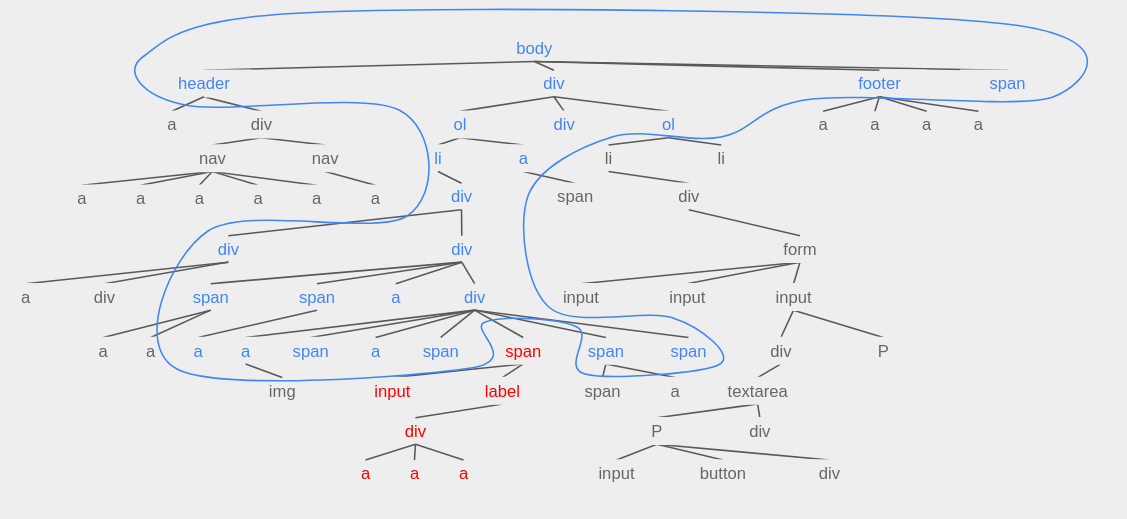
\includegraphics[scale=0.3]{lobsters.png}
\caption{
The Double Dirty Bit algorithm in action
  on a \texttt{lobste.rs} page.
The red \texttt{input} node is being dirtied.
However, to reach the node, Double Dirty Bit have to traverse the 25 blue nodes.
This is typical, especially for
  the most latency-critical user interactions.
}
% https://lobste.rs/s/7ixd88/c_complexity_compiler_bugs
\label{fig:dom-tree-db}
\end{figure}
